\paragraph{Autoren-Bedienoberfläche}
\label{sec:autor_ui}\index{Autoren-Bedienoberfläche}
\ac{aem} ermöglicht es Autoren, ihre Webinhalte über zwei Bedienoberflächen zu gestalten. Dies wäre zum einen die klassische Oberfläche, welche für Desktop-PCs ausgelegt ist, und zum anderen die Touch-optimierte für Tablets und Smartphones. Jeder Autor kann sich eine Oberfläche nach Belieben aussuchen und ggf. nachträglich zur jeweils anderen wechseln.\\
Da die Touch-optimierte Bedienoberfläche nach der Installation von \ac{aem} als Standard eingestellt ist und auch auf dem Desktop-PC lauffähig ist, werden sich die folgenden Kapitel, sofern nicht anders erwähnt, mit dieser Oberfläche befassen. \\
Die Autoren-Bedienoberfläche bietet zahlreiche Werkzeuge, um Webseiten nach Belieben zu gestalten. Dazu gehört der Bearbeitungsmodus für Seiten, zu sehen in \autoref{img:aemui}.

\begin{figure}[H]
	\begin{center}
      	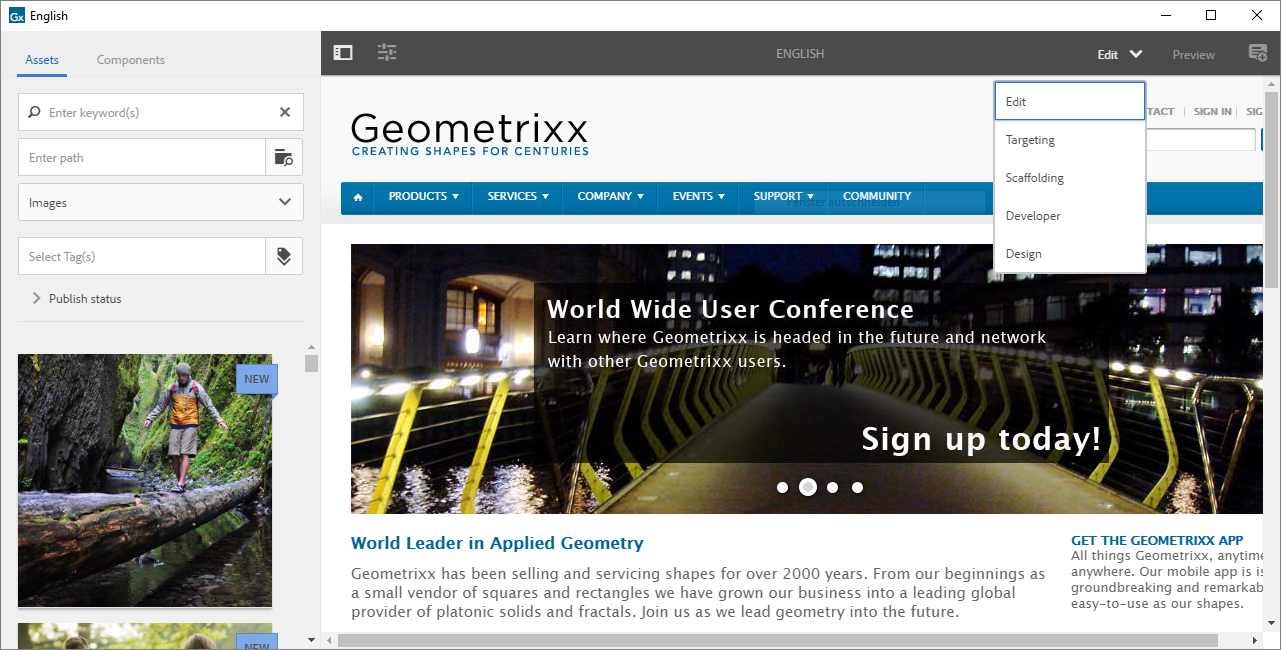
\includegraphics[width=1\textwidth]{aem_autoren_ui.png}
		\caption{Autoren-Bedienoberfläche}
		\label{img:aemui}
	\end{center}
\end{figure}

Das linke Menü lässt sich nach Bedarf auf- und zuklappen. Unterschreitet das Browserfenster eine gewisse Breite, nimmt das Menü dessen gesamte Fläche ein. Hier können Inhalte (Bilder, Dokumente etc. ) und Komponenten durch Ziehen und Loslassen der Seite hinzugefügt werden. In der oberen rechten Ecke wird zwischen verschiedenen Modi gewechselt. Diese sind:

\begin{description}
	\item[Edit:] Inhalte, Texte und Komponenten können eingefügt, entfernt und bearbeitet werden.
	\item[Targeting:] Verwendung des Zusatzproduktes Adobe Target, Teil von \ac{amc}.
	\item[Scaffolding:] Zum Erstellen von mehreren Seiten mit ähnlichem Aufbau.
	\item[Developer:] Für Entwickler, um Komponenten zu debuggen.
	\item[Design:] Hier wird das Design der Seite angepasst.
\end{description}
